\documentclass[]{article}

\usepackage[utf8]{inputenc}

\usepackage[T1]{fontenc}

\usepackage[english]{babel}

\usepackage{amsmath, amsfonts, amssymb, amsthm}

\usepackage{fullpage}

\usepackage{enumerate}
\usepackage{graphicx}
\usepackage{algorithm}
\usepackage{algorithmic}

\usepackage{hyperref}
\hypersetup{
    colorlinks,
    citecolor=black,
    filecolor=black,
    linkcolor=black,
    urlcolor=black
}


%Pour les algos
\floatname{algorithm}{Algorithme}
\renewcommand{\algorithmicrequire}{\textbf{Entrée:}}
\renewcommand{\algorithmicensure}{\textbf{Sortie:}}
\renewcommand{\algorithmicif}{\textbf{si}}
\renewcommand{\algorithmicthen}{\textbf{alors}}
\renewcommand{\algorithmicelse}{\textbf{sinon}}

\title{
{\Huge Speaker classification project}\\
Signal processing\\
}

\author{
\textbf{Dell’Aria Doriano}
\and
\textbf{Goffaux Lionel}\\
}

\date{\today\\
Academic Year 2020-2021\\
Bachelor's degree in Computer Science\\}

\begin{document}

\maketitle
\pagebreak

% \tableofcontents
% \pagebreak

\section{Introduction}
In this project, we are going to extract features of a set of voice samples, to be able to classify if the sample is a
male or female voice.

\section{Energy}
In the \autoref{energy}, we plot the sample and its energy. We observe that with a threshold of 5,
we are able to classify the voiced and unvoiced frames.
Then we use these voiced frames to extract all the features we need.


\begin{figure}[H]
    \centering
    \caption{\label{energy}Energy of a sample}
    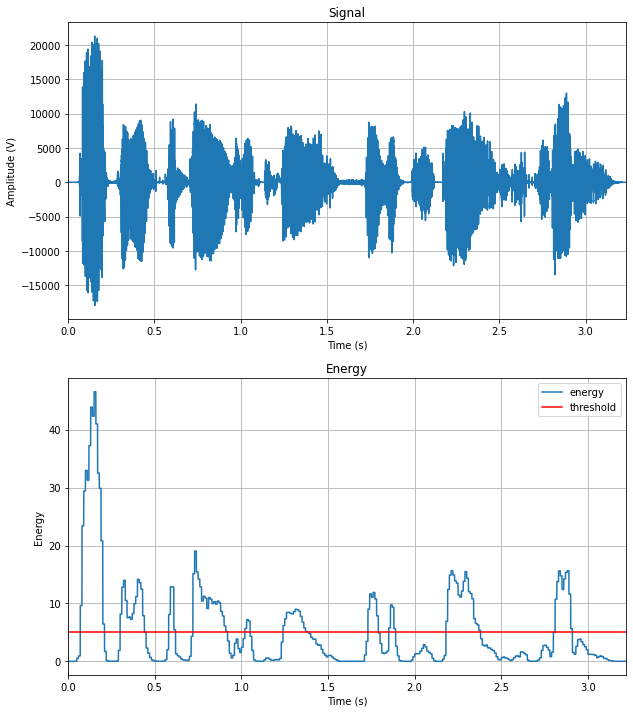
\includegraphics[scale=0.5]{images/energy_threshold.png}
\end{figure}

\section{Features extraction}
\subsection{Pitch}
They are multiple ways to extract the pitch of a sample. In our case, we extract the pitch with an autocorrelation-based
system and a cepstrum-based system.

\subsubsection{Autocorrelation-Based Pitch Estimation System}
The principle of autocorrelation is to correlate the signal with itself. We first split the signal into frames then autocorrelate
frames with themselves.
So we obtain the pitch by measuring the distance between the distance of two peaks of the autocorrelation. 
We fix the frames' width = 21, the step = 5 and the threshold = 5. 
In the \autoref{autocorr}, we observe that the method doesn't have 100\% accuracy because we obtain pitch over 5000 Hz.

\begin{figure}[H]
    \centering
    \caption{\label{autocorr}autocorrelation-based system}
    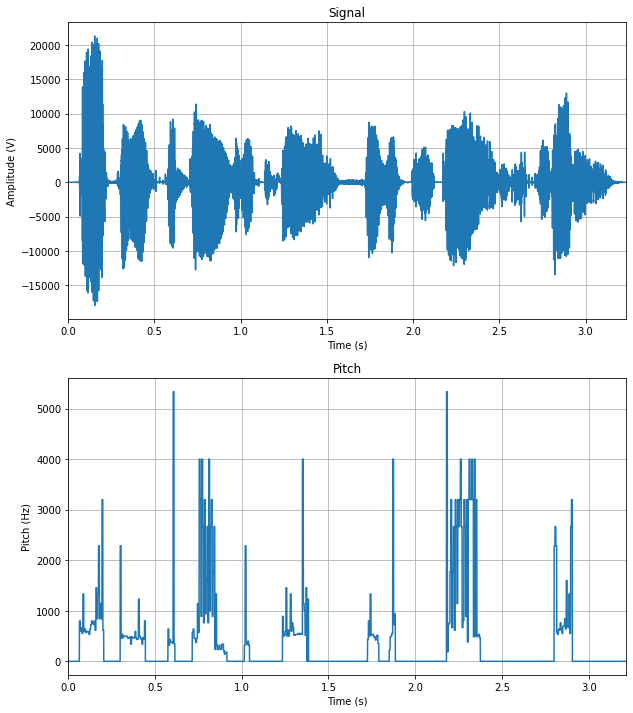
\includegraphics[scale=0.5]{images/autocorr_pitch.png}
\end{figure}

\subsubsection{Cepstrum-Based Pitch Estimation System}
The cepstrum-based pitch estimation system is based on the inverse Fourier transform of the signal's log spectrum.
The signal's log spectrum gives us the frequencies of the initial signal, and the inverse Fourier transform of the signal's log
spectrum gives us the distance between the harmonics of the signal thus we get the fundamental frequency.
We see in the \autoref{cepstrum} that we get better results with that method.

\begin{figure}[H]
    \centering
    \caption{\label{cepstrum}cepstrum-based system}
    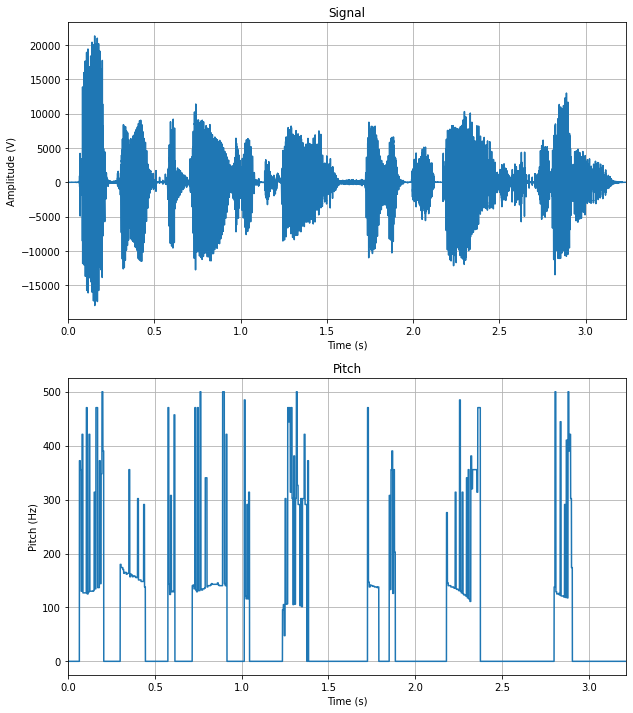
\includegraphics[scale=0.5]{images/cepstrum_pitch.png}
\end{figure}

\subsection{Formants}
The formants are large peaks resulting from the resonance of the vocal tract. We use the linear predictive
coding's roots to obtain the formants. We can see the frequency of the four formants on the \autoref{formants}.

\begin{figure}[H]
    \centering
    \caption{\label{formants}Formants}
    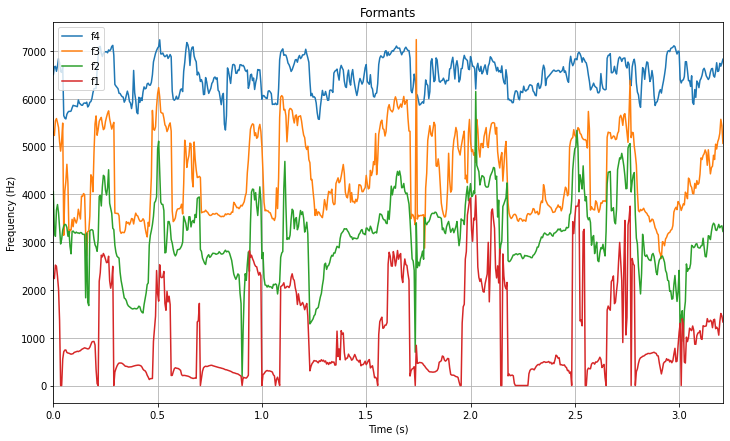
\includegraphics[scale=0.5]{images/formants.png}
\end{figure}

\subsection{Mel-Frequency Cepstral Coefficients (MFCC)}
The coefficients of the MFCC represent the filter of the voice tract. To extract them, we first preprocess the signal by filtering it with a
high pass filter then by applying a Hamming window on it and finally by taking the power spectrum. Then we pass the pre-process signal through
a Mel-filter bank. On the \autoref{fbank}, we can see the Mel filter bank computed for a random sample of voice.

\begin{figure}[H]
    \centering
    \caption{\label{fbank}Mel-filter bank}
    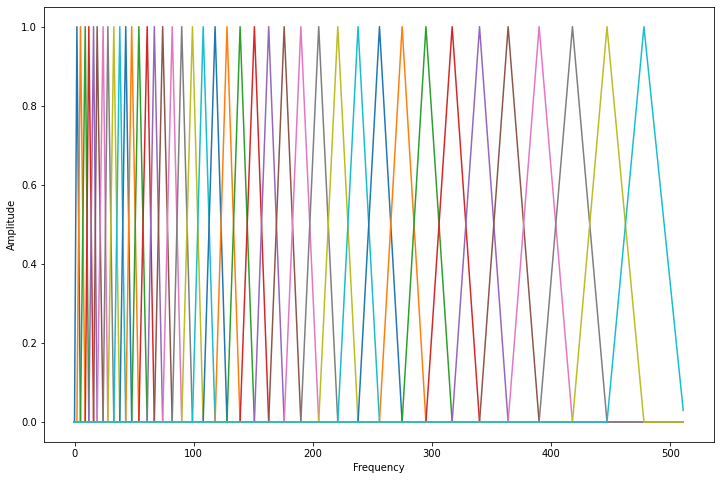
\includegraphics[scale=0.5]{images/fbank.png}
\end{figure}

We can see on the \autoref{mfcc} that the first filter is more triggered than the others.

\begin{figure}[H]
    \centering
    \caption{\label{mfcc}MFCC}
    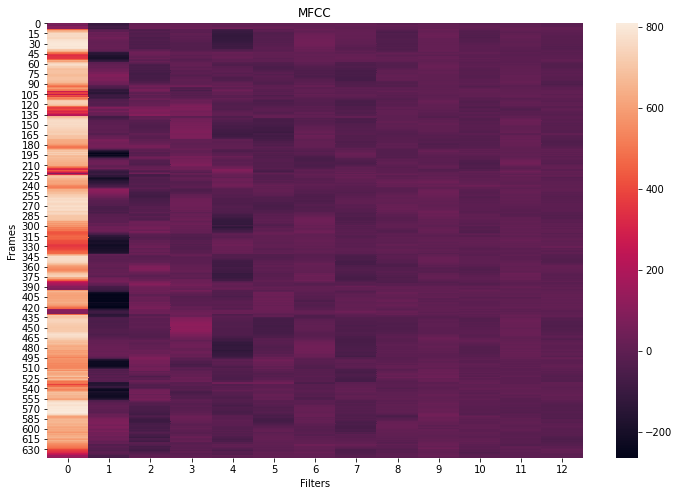
\includegraphics[scale=0.5]{images/mfcc.png}
\end{figure}



% ====== exemple d'algo =======
% \begin{algorithm}
%     \caption{Recherche linéaire du maximum}
%     \begin{algorithmic}[1]
%     \REQUIRE un tableau d’entiers $A$
%     \ENSURE la valeur du plus grand entier contenu dans $A$
%     \STATE $max \leftarrow -\infty$
%     \FOR{$i \leftarrow 1$ `a $longueur[A]$}
%     \IF{$max < A[i]$}
%     \STATE $max \leftarrow A[i]$
%     \ENDIF
%     \ENDFOR
%     \RETURN $max$
%     \end{algorithmic}
% \end{algorithm}


\end{document}